\chapter{Introdução}\label{CAP:introducao}

Este documento descreve o desenvolvimento de um sistema para captação e análise de dados referentes à direção de um motorista.

A ideia básica é coletar dados de sensores já presentes em carros modernos através da porta OBD-II, que utiliza um padrão internacional de disponibilização de informações referentes a um carro [REF 2] e usá-los para definir perfis de direção, ou seja, classificar de alguma forma a forma como uma pessoa dirige.

\section{Motivação}

Qual o perfil de direção de um motorista? Como categorizar os condutores segundo um critério claro?

Buscando responder essas perguntas e, consequentemente, entender as características de pessoas ao volante, este trabalho propõe-se a criar uma infraestrutura de captura e análise de dados em automóveis de uso pessoal.

As informações recolhidas serão armazenadas em uma plataforma de nuvem, protegidas por algum nível de segurança, implementado neste mesmo projeto e, por fim, serão analisadas para gerarem conclusões interessantes sobre o modo de dirigir de cada participante do estudo.
	
Uma pesquisa preliminar sobre o assunto revelou que já existe uma patente para um produto parecido; ela foi registrada em 2013 e avalia o desempenho de um motorista a partir de dados pré-coletados de parâmetros relevantes à condução do carro [REFERENCIA 1].

Visão lateral do carro proposto na patente.[IMAGEM, REF 1]

[CITAR OS TRABALHOS QUE JÁ FAZEM ISSO QUE EU DISSE]

\section{Objetivo}

Este trabalho procura analisar o comportamento de motoristas em situações diversas: no trânsito, em uma prova de direção ou em uma rodovia, por exemplo.

Para isso, fará uso da infraestrutura já presente em carros atuais, conforme pode ser visto na imagem a seguir, mas também pode complementá-la com mais equipamentos, caso seja necessário para o projeto.


\begin{figure}[hp]
    \centering
    
    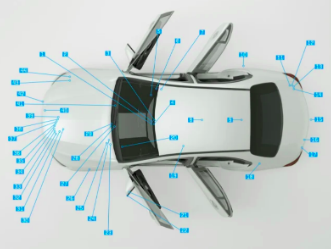
\includegraphics[]{figures/sensores_carro.png}
    
    \caption{Sensores estão presentes em um carro atual na ordem de dezenas[REF 2]}
\end{figure}

Sensores estão presentes em um carro atual na ordem de dezenas[2].

A coleta de dados será feita, a princípio, a partir de ensaios em carros reais feitos por uma quantidade seleta de pessoas, que pode ser expandida para resultados mais precisos na análise posterior.

Os dados coletados deverão ser passados para algum serviço de nuvem, usando conexão à Internet, caracterizando uma aplicação IoT.
	
Do lado da nuvem, será possível utilizar os dados de cada usuário de forma anônima, para diagnosticar o perfil do condutor e possivelmente gerar insights sobre como a pessoa poderia melhorar.
	
A plataforma poderá, após implementada, servir como base de dados para outros projetos futuros, que não farão parte deste TCC, por exemplo:

Prova de direção usando Inteligência Artificial: possível supressão da prova do Detran, avaliando o condutor ao longo das aulas práticas

Seguros de carro personalizados: valores mais altos para motoristas mais violentos

Classificação de motoristas de aplicativo: avaliação ponderada pela forma de dirigir

 
\section{Justificativa}
% ROMEO e PIRES [GIT]
% Pq o trabalho é importante?
No ano de 2021, 11647 pessoas morreram em acidentes de trânsito no Brasil [REF 6], além disso, no mundo inteiro morrem 1,35 milhão de pessoas em média, todos os anos [REF 7], número comparável às mortes por Covid 19 até abril de 2022 [REF 8].

Levando-se em conta esses fatos, é simples entender a relevância deste projeto, pois ele define métricas importantes para classificação da conduta de motoristas, as quais podem ser usadas justamente para evitar acidentes e, portanto, preservar a vida humana.

É possível que no futuro os carros não sejam mais dirigidos por humanos ou que atuem por conta própria na maior parte das situações. Prevê-se, inclusive, que carros com nível de automação de pelos menos 4 comecem a se popularizar em 2025 [REF 9].

Dessa forma, embora o fator humano venha a ser menos relevante para os acidentes do futuro, é preciso também haver métricas para classificar a condução dos veículos autônomos.

Este projeto tem, portanto, extrema relevância, pois é uma possível ferramenta para diminuir as mortes no trânsito, seja causada por pessoas ou por carros autônomos.

\section{Organização do trabalho (antes era "PROCUCAO CIENTIFICA")}

O padrão OBD-II foi uma extensão do padrão OBD-I, uniformizando esse tipo de conector em casos em geral, começando a ser adotado no Brasil a partir de 2010[4].

Nesse padrão de conexão e comunicação é definida uma interface por onde parâmetros internos a um carro podem ser monitorados.

As mensagens definidas pelo OBD-II têm cada uma um PID (parameter ID). O conjunto comum de PIDs de serviços que podem ser solicitados pela porta OBD-II e para que servem pode ser visto na tabela a seguir[REF 3].

[TABELA]

Service / Mode (hex)
Description
01
Show current data - I/M Monitors and Live Data
02
Show Freeze Frame (FF) Data
03
Show Stored Diagnostic Trouble Codes
04
Clear/Erase Diagnostic Trouble Codes and stored values
05
Test results, oxygen sensor monitoring (non CAN only)
06
Test results, other component/system monitoring (Test results, oxygen sensor monitoring for CAN only)
07
Show pending Diagnostic Trouble Codes (detected during current or last driving cycle)
08
Control operation of on-board component/system (EVAP)
09
Request Vehicle Information (VIN)
0A
Permanent Diagnostic Trouble Codes (DTCs) (Cleared DTCs)

É importante notar que os serviços do padrão OBD-II comuns a todos os carros sempre começam com o dígito zero (hexadecimal), por isso, serviços específicos de cada fabricante devem começam a partir do código 0x10.

\begin{figure}[hp]
    \centering
    
    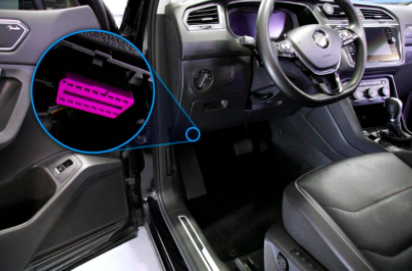
\includegraphics[]{figures/localizacao_obd2.png}
    
    \caption{Posição da porta OBD-II em um carro[REF 5]}
\end{figure}

Os dados que podem ser coletados de qualquer carros são explicitados na tabela abaixo[3]:

[TABELA]

Interessante notar que, embora não esteja representado na tabela, os PIDs 0x00, 0x20, 0x40, etc, ou seja, a cada 32 valores de PID, existe um parâmetro apenas para indicar quais entre os PIDs seguintes são fornecidos por aquele carro.

Esses PIDs de marcação, por assim dizer, utilizam 4 bytes para comunicar quais dos próximos PIDs estão disponíveis, utilizando cada bit como uma flag binária. 

Na imagem a seguir é possível visualizar como esse processo é feito, usando como exemplo o valor 0xBE1FA813 para representar os 4 bytes oferecidos[REF 3].

\begin{figure}[hp]
    \centering
    
    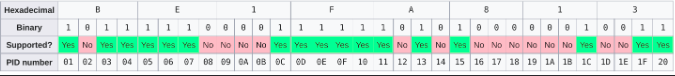
\includegraphics[scale=0.7]{figures/tabela_dados_disponiveis.png}
    
    \caption{}
\end{figure}


\section{Organização da tese}

\noindent \textbf{Capitulo \ref{CAP2}}: descricao...

\noindent \textbf{Capitulo \ref{CAP3}}: descricaoo...

\noindent \textbf{Capitulo \ref{CAP4}}: descricao...

\noindent \textbf{Capitulo \ref{CAP5}}: descricao...